\documentclass[a4paper,11pt]{article}

\usepackage[T1]{fontenc}
\usepackage[french]{babel}
\usepackage[utf8x]{inputenc}
%\usepackage{palatino} %change la police d'écriture.
\usepackage{lipsum} %pour avoir un texte, en latin, déja écrit, inutile dans 99,999999 % du temps.


%modules mathématiques :
\usepackage{amsmath}
\usepackage{amssymb}
\usepackage{mathrsfs} %pour avoir un police d'écriture anglo-saxonne en mode mathématique.
\usepackage{amsthm}
\usepackage{amssymb} %symboles en plus.
\usepackage{amsfonts}

%autres packages :
\usepackage{verbatim} %pour pouvoir changer de police dans le document.
\usepackage{mathptmx} %pour utiliser une autre police
\usepackage{dsfont}
\usepackage{graphicx} %pour pouvoir faire des graphes.
\usepackage{color} %pour mettre de la couleur
\definecolor{bblack}{cmyk}{0,0,0,1} 
\usepackage[colorlinks=true,linkcolor = black,urlcolor=black]{hyperref} %pour les liens hypertextes
% \usepackage{Sweave} %pour du code R
% \usepackage{mhchem}
%si on veut mettre du code python
\usepackage{listings}
\definecolor{dkgreen}{rgb}{0,0.4,0}
\definecolor{gray}{rgb}{0.5,0.5,0.5}
\definecolor{mauve}{rgb}{0.58,0,0.82}
\definecolor{dkyellow}{cmyk}{0, 0, 0.2, 0}
\lstset{
  language=Python,                % the language of the code
  basicstyle= \footnotesize,      % the size of the fonts that are used for the code
  numbers=left,                   % where to put the line-numbers
  numberstyle=\tiny\color{gray},  % the style that is used for the line-numbers
  stepnumber=2,                   % the step between two line-numbers. If it's 1, each line 
                                  % will be numbered
  showspaces=false,               % show spaces adding particular underscores
  showtabs=false,                 % show tabs within strings adding particular underscores
  frame=single,                   % adds a frame around the code
  rulecolor=\color{black},        % if not set, the frame-color may be changed on line-breaks within not-black text (e.g. commens (green here))
  tabsize=2,                      % sets default tabsize to 2 spaces
  captionpos=b,                   % sets the caption-position to bottom
  breaklines=true,                % sets automatic line breaking
  breakatwhitespace=false,        % sets if automatic breaks should only happen at whitespace
  keywordstyle=\color{blue},      % keyword style
  commentstyle=\color{dkgreen},   % comment style
  stringstyle=\color{mauve},       % string literal style
  backgroundcolor=\color{dkyellow},      % choose the background color. You must add \usepackage{color}
}
%%%%%%%%%%%%%%%%%%%%%%%%%%%

%%%%%% Pour reduire les marges ! %%%%%%%%%%%%%%%
\setlength{\textwidth}{15cm} %Largeur du texte : n
%\setlength{\marginparwidth}{0cm}
\setlength{\oddsidemargin}{0.5cm} %m avec 2m+n = 16 pour que ca marche bien.
%\setlength{\headheight}{0cm}
%\setlength{\topmargin}{2cm} %hauteur marge d'en haut
%\setlength{\headsep}{0cm} %hauteur de l'en tete
%\setlength{\textheight}{21cm} %hauteur du texte
%\setlength{\footskip}{0cm} %hauteur du pied de page
%\setlength{\marginparsep}{0cm}
%%%%%% Commandes pour structurer le texte %%%%%%%
%\part
%\section
%\subsection
%\subsubsection

%Pour énumérer, dans une section ou une sous-section :
%\begin{enumerate}
%\item texte
%\item texte2 etc.
%\end{enumerate}

%\vspace{n pt} : met un espace de n point(s) entre les paragraphes. Attention à l'utilisation.
%\vspace{6 ex} : met un espace de 6 hauteurs de police entre les paragraphes. Attention à l'utilisation.
%\vspace*{...} : force l'espace, même si c'est au début ou à la fin d'une page. Tres attention a l'utilisation.

% \\ pour passer une ligne
% \newpage pour écrire ce qui suit sur une nouvelle page
% \clearpage : pour ne rien ecrire de plus sur la page en cours

%%%%%%%%%%%%%%%%%%%%%%%%%%%%%%%%%%%%%%%%%%%%%%%%%%

%%%%%%%%%%%%% Deux modes maths %%%%%%%%%%%%%%%%%%%
% mettre entre $, ex : $ 2+2 = 4$ 
% mettre entre \[ \], ex : \[ 2+2 = 4 \].
%Attention, rendus différents
%%%%%%%%%%%%%%%%%%%%%%%%%%%%%%%%%%%%%%%%%%%%%%%%%%

%%%%%%%%%%%%Pour faire un calcul, centré sur les = %%%%%%%%%%%%%%%
%\begin{align*}
%calcul, tout sera déja en mode maths.
%a &= b
%&= c+d-E etc.
%\end{align*}
%%%%%%%%%%%%%%%%%%%%%%%%%%%%%%%%%%%%%%%%%%%%%%%%%%



%%%%%%%%%%%% Pour mettre en valeur un résultat %%%%%%%%%%%%%%%%%%%
%\begin{abstract}
 %résultat\begin{abstract}
%\end{abstract}
% Attention au rendu, il faudrait réussir à enlever la phrase en gras juste au dessus.
%%%%%%%%%%%%%%%%%%%%%%%%%%%%%%%%%%%%%%%%%%%%%%%%%%%%%%%%%%%%%%%%%%%

%%%%%%%%%%%% Pour des références %%%%%%%%%%%%%%%%%%%%
%\label{ref1}
%\ref{ref1}
%\pageref{ref1}
%%%%%%%%%%%%%%%%%%%%%%%%%%%%%%%%%%%%%%%%%%%%%%%%%%%%%

%%%%%%%%%%%% Pour des fleches stylees %%%%%%%%%%%%%%%
%\xrightarrow[nce qu'il y aura en dessous]{ce qu'il y aura au dessus}
%ex :\xrightarrow[n \to \infty]{P-ps}
%%%%%%%%%%%%%%%%%%%%%%%%%%%%%%%%%%%%%%%%%%%%%%%%%%%%%


%%%%%%%%%%% Pour rajouter des trucs en dessous (au dessus d'une expression) %%%%%%%%%%%%%%%%%%
%\underset{ce qu'il y a en dessous}{ce qu'il y a au dessus}
%\underset{n\to \infty}{=}

%\overset{ce qu'il y a au dessus}{ce qu'il y a en dessous}
%\overset{n\to \infty}{=}
%%%%%%%%%%%%%%%%%%%%%%%%%%%%%%%%%%%%%%%%%%%%%%%%%%%%%%

%%%%%%%%%%% Pour inclure un graphique %%%%%%%%%%%%%%%%
%\includegraphics[hauteur]{nom de l'image} % L'image doit être dans le même fichier que le fichier.tex.
%ex : \includegraphics[width=11cm]{unif_n10.jpeg}
%%%%%%%%%%%%%%%%%%%%%%%%%%%%%%%%%%%%%%%%%%%%%%%%%%%%%%
                    
                     
% mathbb pour les corps R, C ...
% mathcal pour les lettres caligraphiques (tribus etc.)
% mathfrak pour les lettres ghotiques
% mathbf pour les lettres en gras

%%%%%%%%%%%% Pour le titre la date et autres infos du pdf %%%%%%%%%%%%%
% \title{Book Report on : Heat Wave}
% \author{Benjamin Donnot}
% \date{}

%\pdfinfo{%
%  /Title    ()
%  /Author   ()
%  /Creator  ()
%  /Producer ()
 % /Subject  ()
%  /Keywords ()
%}
%%%%%%%%%%%%%%%%%%%%%%%%%%%%%%%%%%%%%%%%%%%%%%%%%%%%%%%%%%%%%%%%%%%%%%%%%%

%%%%%%%%%%%%%%%%%%%%%%% Affichage du titre ou autre %%%%%%%%%%%%%%%%%%%%%%
% \maketitle : affiche le titre
%%%% \tableofcontents : pour faire une table des matières
%%%%%%%%%%%%%%%%%%%%%%%%%%%%%%%%%%%%%%%%%%%%%%%%%%%%%%%%%%%%%%%%%%%%%%%%%%

%%%%%%%%%%%%Pour des entetes stylees%%%%%%%%%%%%%%%%%%%
\makeatletter
\def\clap#1{\hbox to 0pt{\hss #1\hss}}%
\def\ligne#1{%
\hbox to \hsize{%
\vbox{\centering #1}}}%
\def\haut#1#2#3{%
\hbox to \hsize{%
\rlap{\vtop{\raggedright #1}}%
\hss
\clap{\vtop{\centering #2}}%
\hss
\llap{\vtop{\raggedleft #3}}}}%
\def\bas#1#2#3{%
\hbox to \hsize{%
\rlap{\vbox{\raggedright #1}}%
\hss
\clap{\vbox{\centering #2}}%
\hss
\llap{\vbox{\raggedleft #3}}}}%
\def\maketitle{%
\thispagestyle{empty}\vbox to \vsize{%
\haut{}{\@blurb}{}
\vfill
\vspace{1cm}
\begin{flushleft}
\usefont{OT1}{ptm}{m}{n}
\huge \@title
\end{flushleft}
\par
\hrule height 4pt
\par
\begin{flushright}
\usefont{OT1}{phv}{m}{n}
\Large \@author
\par
\end{flushright}
\vspace{1cm}
\begin{center}
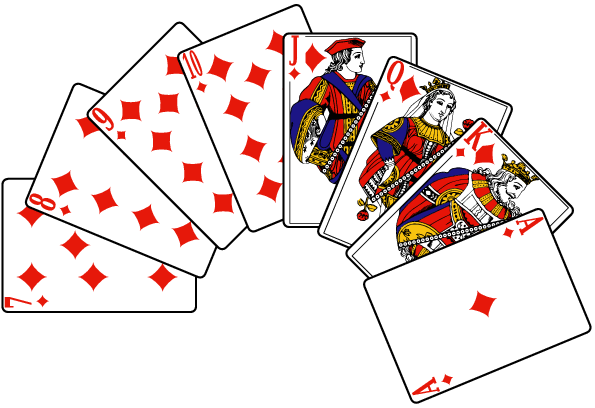
\includegraphics[width=13cm]{belote.jpg}
\end{center}

\vfill
\vfill
\bas{}{}{}
}
\cleardoublepage
}
\def\date#1{\def\@date{#1}}
\def\author#1{\def\@author{#1}}
\def\title#1{\def\@title{#1}}
\def\location#1{\def\@location{#1}}
\def\blurb#1{\def\@blurb{#1}}
\date{\today}
\author{}
\title{}
\location{}\blurb{}
\makeatother
\title{Projet de C++ débutant : la Belote}
\author{Morgane AUSTERN \\
Benjamin DONNOT\\
Loïc MICHEL}
\location{}
\blurb{}

\renewcommand{\thesection}{\Roman{section}}
\renewcommand{\thesubsection}{\arabic{subsection}}
\renewcommand{\thesubsubsection}{\roman{subsection}}
%%%%%%%%%Pour l'en-tete et le pied de page%%%%%%%%%%%%%%%%%%
\usepackage{fancyhdr}
\pagestyle{fancy}
\usepackage{lastpage}
\renewcommand\headrulewidth{1pt}
\renewcommand\footrulewidth{1pt}
\fancyfoot[C]{Benjamin DONNOT \\ \textbf{Page \thepage/\pageref{LastPage}}}
\fancyfoot[R]{ Loïc MICHEL}
\fancyfoot[L]{Morgane AUSTERN}

\begin{document}
\maketitle
\tableofcontents
\clearpage
\section*{Introduction}
\addcontentsline{toc}{section}{Introduction} 
%Taper l'introduction ici : %
L'année dernière certains d'entre nous avons fait notre projet de python sur un autre jeu de carte, le jeu de Tarot. Il restait de nombreuses pistes d'améliorations que nous avons essayé de mettre en \oe{}uvre dans ce projet de C++. Nous avons donc décidé de coder un jeu différent du tarot mais tout de même relativement proche : le jeu de belote. \\

Nous avons entre autre tenté d'améliorer l'intelligence artificielle, et l'interface graphique. Pour l'amélioration de l'intelligence artificielle, nous avons tenté de mettre en place des méthodes de "machine learning". Mais ceci n'a pas été évident car nous avons rencontré de nombreux problèmes quant à la lecture et écriture de données dans des fichiers avec c++.
\clearpage
\section{Le jeu}
Le jeu de Belote comporte de nombreuses variantes. Nous n'avons retenu ici que la belote "classique". C'est à dire qu'on ne joue pas à la Belote "coinchée". Nous ne prenons pas non plus en compte les annonces.\\

La difficulté du jeu de Belote est multiple : la hauteur de deux cartes ne suffit pas à déterminer laquelle est "plus forte" que l'autre. En effet, à la belote l'atout est choisi en début de partie et est déterminé pour toute la manche. L'ordre des cartes n'est pas le même si une carte est une carte "simple" ou un atout. Pour contourner ce problème, nous avons rajouté un attribut "atout"\footnote{"trump" en anglais} dans la classe jeu (classe qui structure le programme). Cet attribut est renvoyé dans quasiment toutes les méthodes des autres classes appelées par cette classe. \\

Une autre difficulté du jeu de Belote est la complexité des règles qui autorise à jouer une carte donnée dans une situation donnée. Il faut jouer dans le couleur demandée (hauteur de la première carte jouée dans le pli) si on en possède, sinon on doit couper. Il est cependant possible de ne pas couper si le partenaire est maitre ou si on n'a plus d'atouts en notre possession. Ceci a été assez complexe à faire interpréter à l'ordinateur, car les enchainements de conditions ne sont pas forcément triviaux. \\

L'aspect jeu comporte également un enchainement d'actions à faire réaliser par un joueur spécifique (jouer une carte, remporter le pli, dire s'il veut prendre etc.) Cet enchainement précis a également posé, au début, quelques petites difficultés. Ces difficultés ont été encore une fois surmontées grâce à la "programmation orientée objet" et à la possibilité de rajouter un attribut à la classe Jeu : un attribut pour savoir quel joueur devra donner au prochain tour et un autre pour déterminer quel joueur devra effectuer l'action en cours (jouer une carte ou décider s'il doit prendre par exemple). Ces deux attributs sont incrémentés et décrémentés au fur et à mesure du déroulement d'une partie.\\

La classe jeu est donc l'ossature du programme. Elle gère l'enchainement des toutes les actions et fait évoluer le jeu en fonction des informations reçues par les autres classes.
\clearpage
\section{Joueurs}
Si la classe jeu est chargée de procéder au bon déroulement des différentes actions, c'est bien la classe joueur qui est chargé de prendre les décisions. Et très vite nous nous sommes rendu compte que les décisions pouvaient être de deux types : soit l'ordinateur les prends tout seul (c'est le cas des joueurs IA) soit un humain doit les prendre.\\

Afin de régler une fois pour toute ce problème nous avons décidé de faire hériter de la classe 'joueur' deux classes : une pour les joueurs qui seront gérés par l'ordinateur (Joueur$\_$IA), et l'autre pour les joueurs humains (Joueur$\_$Humain). \\

Avec le raisonnement ci-dessus, il est clair qu'un "joueur simple" n'existe pas. Donc pour éviter de faire jouer un joueur simple, nous avons choisi de faire de la classe 'Joueur' une classe virtuelle pure. Là encore la programmation orientée objet permet de sous-traiter la prise de décision aux deux "sous-classes", en appelant les méthodes adaptées via un pointeur sur Jouer, qui pointera soit sur une instance de Joueur$\_$Humain soit sur une instance de Joueur$\_$IA.\\

\'A l'instart de la classe 'Jeu' la classe 'Joueur' sert donc uniquement à structurer les données et à renvoyer ce qu'il faut à la classe jeu pour qu'une partie puisse se dérouler sans accrocs majeurs. Ce n'est qu'une interface entre le jeu et les différents types de joueurs présents.
\subsection{Les joueurs gérés par l'ordinateur}
Dans cette classe, toutes les décisions sont prises par l'ordinateur. Il a donc fallu lui apprendre à jouer de façon non complètement triviale. En effet, une IA\footnote{Intelligence Artificielle} qui choisit une carte aléatoirement ou encore décide au hasard de prendre ou de ne pas prendre n'est pas très performante et se fera battre à coup sûr par un joueur humain, même débutant. Un tel jeu ne présenterait pas énormément d'intérêt.\\

Une fois encore, les décisions prises par l'ordinateur peuvent être de types. Soit l'ordinateur doit choisir s'il prend ou pas, soit il doit choisir une carte à jouer. 
\subsubsection{Prendre ou ne pas prendre, telle est la question}
La première étape la prise décisionnelle, le choix de la prise, est assez "simple". Il suffit de renvoyer un booléen : je prends/je ne prends pas ou éventuellement une couleur à laquelle l'IA veut prendre.\\

Pour se faire nous avons choisi d'évaluer le score moyen que l'ordinateur peut espérer obtenir en fin de partie s'il a choisi l'atout et de lui faire prendre à cette couleur si ce score est "raisonnable". Pour évaluer le score moyen espéré plusieurs solutions s'offraient à nous. Nous avons décidé d'attribuer des scores à chaque particularité du jeu (nombre d'atouts, nombre d'as, nombre de 10, existence d'une longe etc.) Toutes ces particularités sont passées en revues par l'ordinateur qui va ensuite évaluer le nombre de points espérés. Si ce score est supérieur à un seuil minimal, le joueur prend, sinon il ne prend pas. \\

Pour améliorer ce processus, nous avons décidé d'implémenter une stratégie de "machine learning" .Ceci consiste globalement à récupérer les données qui affectent le score à la création du joueur IA (intensité de modification du score). Et, en fonction de l'issue (gain ou perte) de la partie, les données seront modifiées : plus la différence entre le score de l'équipe du joueur concernée et celle de l'équipe adverse est grande, plus les scores en question se verront augmenter. Ces scores se verront également diminuer d'une manière similaire en cas de perte. Ceci permet à tous les joueurs IA de profiter de l'expérience acquise par le joueur qui a pris. Hélas au moment où le code a été envoyé cette fonctionnalité n'était pas encore tout a fait opérationnelle. Elle le sera pour la présentation.\\

Une piste d'amélioration de cette méthode serait de définir différents types de joueurs IA en rajoutant un attribut "type" et qui permettrait de charger au départ des données différentes. Ceci aurait présenté l'avantage de pouvoir faire des joueurs plus ou moins agressifs (ou ayant des comportements plus ou moins rationnels) et ensuite de les faire se "battre" entre eux sur de nombreuses manches pour savoir quelle stratégie l'emporte. Une autre application aurait été de pouvoir voir comment les données d'un joueur évoluent au cours des parties jouées et s'il y a "convergence" des-dites données.\\

Les gros inconvénients de ces méthodes résident dans le fait que la structure des cas envisagés est rigide : il n'est pas possible à l'ordinateur d'en rajouter un, même si ce cas a été oublié dans la programmation alors qu'il s'avère important. Un autre inconvénient réside dans la possibilité que le comportement des joueurs peut 'diverger'. Il est en effet tout à fait possible qu'il n'y ait pas de "force de rappel" suffisamment importante pour qu'un score ne croisse pas de façon incontrôlée.
\subsubsection{Quelle carte jouer ?}
Concernant le choix de la carte une méthode similaire mais néanmoins plus compliquée a été implémentée. En effet, le choix de la prise se résume globalement à renvoyer un booléen. Pour jouer c'est un peu plus compliqué. Il faut renvoyer une carte parmi tout un choix possible de cartes jouables\footnote{une méthode spécifique est chargée de déterminer si une carte peut ou non être jouée}. \\

Pour se faire nous avons implémenté une méthode qui permet d'attribuer un score à chacune des cartes jouables et de retenir la carte avec le score le plus important. Le score se voit modifier selon différents paramètres qui l'affecte positivement ou négativement.\\

Là encore c'est notre expérience personnelle qui nous a permis d'isoler les quelques cas possibles qui vont affecter le score. Et, cette approche ne nous permet pas d'en changer. Nous pourrons toujours rajouter des cas manuellement, mais l'ordinateur n'en ajoutera pas seul.\\

L'intensité des modifications du score est ici aussi chargée dans un tableau à la création du joueur IA. Et il serait possible de l'affecter de la même façon que le choix de prendre ou de ne pas prendre. Ce qui diffère cependant c'est la difficulté d'évaluation d'un coup donné.\\

Si le fait de prendre ou pas se révèle judicieux ou non est facile à savoir : si on gagne, le choix était le bon, si on perd il ne l'était pas. \'Evaluer la pertinence du choix d'une carte peut se révéler beaucoup plus complexe et faire appel à nettement plus d'informations. La belote se joue en équipe, il faut donc à la fois tenir compte du signal envoyé à notre partenaire en maximisant l'information qu'on lui transmet, tout en minimisant l'information transmise à nos adversaires. C'est ainsi que nous ne pouvons savoir s'il était judicieux d'avoir joué une telle carte à un pli donné que deux ou trois plis plus tard. Compte tenu de cette difficulté supplémentaire et du peu de temps qu'il nous restait, nous avons donc choisi de ne pas modifier l'intensité des modifications du score attribué aux cartes lorsqu'on doit en jouer une.
\clearpage
\subsection{Les Joueurs Humains}
Les problèmes rencontrés pour la conception de la classe 'Joueur$\_$Humain' sont de natures totalement différentes. En effet, il ne s'agit plus de faire choisir l'ordinateur, mais de lui faire comprendre que le joueur derrière son écran veut effectuer telle ou telle action. L'essentiel de cette classe est donc de renvoyer des informations à la classe 'Joueur' sur ce que le joueur humain a décidé de faire.\\

Les problèmes rencontrés ici sont donc surtout des problèmes liés à la librairie SDL. Il a fallu faire plusieurs classes de d'images avec lesquelles le joueur humain pouvait interagir (boutons ou carte sur lesquels cliquer par exemple).\\

Tout d'abord la classe 'Images' représente une image au sens générique, c'est à dire tout élément susceptible d'être affiché à l'écran. De cette classe hérite deux autres classes : 'Text' dont la principale fonction est d'afficher du texte et 'Button' dont la principale fonction est de changer de couleur lorsque la souris est dessus\footnote{La possibilité de cliquer sur n'importe quelle image est en effet offerte par la classe 'Images'.}.

Les principaux problèmes rencontrés avec SDL sont liés à son intégration plutôt mauvaise dans des classes. En effet, toute 'surface' est en réalité un pointeur sur surface. Pour intégrer ces pointeurs à des classes il faut donc modifier le destructeur pour ne pas que notre programme ait des fuites mémoires. Et, il faut alors également modifier le constructeur copie et l'opérateur 'asignment' pour ne pas avoir de problèmes. Mais pour se faire il faut également garder en mémoire, entre autre, le chemin d'accès à l'image car à notre connaissance, la librairie SDL ne possède pas de méthode permettant de dupliquer une surface sans avoir à la recharger depuis le fichier de base.
\clearpage
\section{TortoiseSVN}
Pour faire ce projet nous avons utilisé un logiciel qui gère les versions. Il s'agit de RapidSVN qui est intégré à Windows via TortoiseSVN.\\

Ceci nous a été très utile pour se transmettre le code que nous pouvions ainsi modifié à notre guise sans pour autant harceler les autres pour avoir la dernière version qu'il venait de coder. De plus, le code étant hébergé sur internet\footnote{ sur le site \href{https://www.assembla.com/start}{Assembla.com}}. Ceci a permis de coder sur plusieurs ordinateurs simultanément et sans se préoccuper des autres. A chaque fois que nous voulions programmer il suffisait de 'updater' pour obtenir la dernière version du code, de la modifier à notre guise puis, avant de 'commit' de remettre à jour notre version du code pour que tout se passe bien. Ceci a nécessité un petit coût d'entrée mais s'est révélé payant sur le 'long terme'.\\

Outre cet avantage nous pouvons également citer le fait de pouvoir revenir aux versions antérieures. Ceci c'est avéré utile quand nous partions sur de fausses pistes ou lorsque le code se mettait à bugguer 'mystérieusement'\footnote{bugs souvent dus à une mauvaise manipulation d'un des codeurs}. Nous pouvions ainsi comparer la version actuelle à la version précédente et avoir une idée d'où les bugs pouvaient venir. Les corriger s'est donc avérer moins 'douloureux' que si un tel outil n'avait pas été employé.
\clearpage
\section{CodeBlocks, Conclusion}
Comme nous trouvions plus agréable de coder avec CodeBlocks (auto complétion -entre autre) et pour des raisons d'affinité d'au moins un de nous avec le monde des licences libres et de la communauté Linux en général nous avons décidé de codé avec CodeBlocks. \\

Nous ne pensions pas avoir de problèmes de compatibilité avec Visual Studio. Ceci était sans compter sur SDL... En effet, il semble que les en-têtes pour inclure SDL ne sont pas les mêmes avec les deux logiciels. Ceci explique donc que nous n'ayons pas pu tester que le projet Visual Studio que nous avons joint aux fichiers que nous vous avons envoyé. Car celui-ci n'a pas réussi à compiler normalement.\\
Nous espérons que cela ne vous posera pas trop de problèmes et nous nous excusons pour la gêne occasionnée.\\

En conclusion, les problèmes que nous avons rencontrés ont été de natures assez différentes. Mais, grâce à la programmation orientée objet et de nombreuses recherches sur internet nous avons réussi à en franchir une bonne partie. \\
\end{document}